\newpage
\setcounter{figure}{0}

\section{Pregled korištenih tehnologija i algoritama} % (fold)
\label{sec:Tehnologija i teorija}


\subsection{Microsof Kineckt 3D kamera} % (fold)
\label{sub:Microsof Kineckt 3D kamera}

% subsection Microsof Kineckt 3D kamera (end)

\subsection{ROS biblioteka i alati} % (fold)
\label{sub:ROS biblioteka i alati}

% subsection ROS biblioteka i alati (end)

\subsection{Biblioteka Pointcloud} % (fold)
\label{sub:Biblioteka Pointcloud}

% subsection Biblioteka Pointcloud (end)


\subsection{Istovremena lokalizacija i mapiranje} % (fold)
\label{sub:Slam}

% subsection Slam (end)

\newpage
\subsection{Poisson algoritam za rekonstrukciju površine} % (fold)
\label{sub:Poisson}
Poisson algoritam za rekonstrukciju
površine~\cite{Kazhdan:2006:PSR:1281957.1281965} razvijen je suradnjom
Michaela Kazhdana i Matthewa Bolitha s Johns Hopkins sveučilišta u
Baltimoru i Huguesa Hoppea iz Microsoft Researcha u Redmondu. Također
Kazhdan i Bolitho su implementirali\footnotemark[1] Poisson algoritam i
objavili kod pod BSD licencom. Na osnovu tog rada algoritam je dodan i u
PCL biblioteku.

U ovom poglavlju dana je osnovna ideja i kratak matematički pregled
algoritma. Opisano je ograničenje algoritma te parametri kojima se može
upravljati rekonstrukcija površine.

\footnotetext[1]{%
Originalna implementacija Poisson algoritma se nalazi na 
\url{http://www.cs.jhu.edu/~misha/Code/PoissonRecon/Version5.5/}}

Rekonstrukcija 3D površina iz uzorka točaka je dobro proučavan problem u
računalnoj grafici. Ona omogućava namještanje skeniranih
podataka, ispunjavanje površinskih rupa i ponovnu izgradnju postojećih
modela.

Poisson algoritam pristupa problemu rekonstrukcije površine rješavanjem
Poissonove jednadžbe. To čini upotrebom metode implicitne funkcije.
Točnije računanjem 3D indikacijske funkcije \(\chi\) (definiranom s 1 u
točkama unutar modela, odnosno s 0 u točkama izvan) i dohvaćanjem
rekonstruktruirane površine izvlačenjem odgovarajuće iso-površine.

Algoritam se oslanja na ideju da postoji cjelovita veza između
orijentiranih točaka uzetih s površine modela i indikacijske funkcije
modela. Točnije, gradijent indikacijske funkcije je polje vektora koje
je uglavnom popunjeno nulama (jer je indikacijska funkcija uglavnom
konstantna), osim kod točaka blizu površine gdje je jednako unutrašnjim
normalama površine. Stoga, uzorci orijentiranih točaka mogu biti
promatrani kao gradijent modelove indikacijske funkcije kao što je
prikazano na slici~\ref{fig:poisson-reconstruction.png}

\begin{figure}[h]
\centering
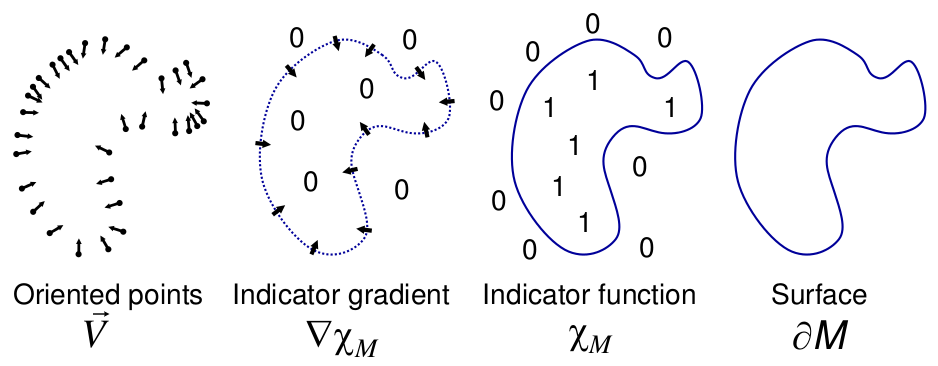
\includegraphics[scale=0.35]{figures/poisson-reconstruction.png}
\caption{Prikaz Poisson rekonstrukcije u 2D}
\label{fig:poisson-reconstruction.png}
\end{figure}

Problem računanja indikacijske funkcije se svodi na invertiranje
operatora gradijenta, odnosno pronalazak funkcije skalara \(\chi\) čiji
gradijent najbolje aproksimira polje vektora \(\vec{V}\) definirano
uzorcima, odnosno 
\begin{equation*}
min_\chi \|\nabla\chi - \vec{V}\|.
\end{equation*}
Ako se primjeni operator divergencije, tada se taj problem pretvara u
standardni Poissonov problem: računanje funkcije skalara \(\chi\) čiji
laplasijan (divergencija gradijenta) je jednak divergenciji polja
vektora \(\vec{V}\),

\begin{equation*}
\Delta \chi \equiv \nabla \cdot \nabla\chi = \nabla \cdot \vec{V}.
\end{equation*}.

Predstavljanje rekonstrukciju površine kao Poissonov problem pruža
nekoliko prednosti. Mnoge implicitne metode namještanja površina
segementiraju podatke u regije za lokalno namještanje i onda te lokalne
aproksimacije spajaju upotrebom funkcija stapanja. Za razliku od njih,
Poisson rekonstrukcija je globalno rješenje koje razmatra sve podatke
odjednom, bez upotrebe heurstičkih podijela i stapanja. Zbog toga
Poisson rekonstrukcija kreira izrazito glatku površinu koja robusno
aproksimira šumovite podatke.  


% subsection Poisson (end)

% section Tehnologija i teorija (end)
